\section{Kalman Filter}

The Kalman filter is applied to estimate the state \( \mathbf{x}(t) \) 
of the system by combining the predicted state from the accelerometer data
with the corrected state from the position measurements.

\subsection{Algorithm}

\textbf{Step 1: Initialization}

The initial state estimate \( \hat{\mathbf{x}}_0 \) is typically set to the expected 
initial position and velocity, i.e., \( \hat{\mathbf{x}}_0 = \mathbb{E}[\mathbf{x}_0] \). 
The initial state covariance \( P_0 \) represents the uncertainty in the initial estimate 
and is usually set to a large value to reflect high uncertainty about the initial state.

\begin{align}
    \hat{\mathbf{x}}_0 &= \mathbb{E}[\mathbf{x}_0] \\
    P_0 &= \mathbb{E}[(\mathbf{x}_0 - \hat{\mathbf{x}}_0)(\mathbf{x}_0 - \hat{\mathbf{x}}_0)^T]
\end{align}

\textbf{Step 2: Prediction Step}

In the prediction step, the state is predicted using the previous state 
estimate and the measured acceleration \( a_k \):

\begin{align}
    \mathbf{x}_{k|k-1} &= A \mathbf{x}_{k-1|k-1} + B a_k \\
    P_{k|k-1} &= A P_{k-1|k-1} A^T + Q
\end{align}

\textbf{Step 3: Update Step}

In the update step, the state estimate is corrected using the position measurement \( y_k \):

\begin{align}
    S_k &= C P_{k|k-1} C^T + R \\
    K_k &= P_{k|k-1} C^T S_k^{-1} \\
    \mathbf{x}_{k|k} &= \mathbf{x}_{k|k-1} + K_k (y_k - C \mathbf{x}_{k|k-1}) \\
    P_{k|k} &= (I - K_k C) P_{k|k-1} (I - K_k C)^T + K_k R K_k^T
\end{align}

\subsection{Simulation Results}

The accelerometer data (\( a_k \)) and position measurements (\( y_k \)) 
were obtained at discrete time steps. Both measurements are sampled at the 
same frequency, with the sampling interval \( \Delta t = 0.01 \, \text{s} \) 
(100 Hz sampling rate). The following values were used to generate the figure:

\textbf{Physical Parameters:}
\begin{itemize}
    \item Mass: \( m = 1.0 \, \text{kg} \)
    \item Damping coefficient: \( c = 0.5 \, \text{N·s/m} \)
    \item Spring constant: \( k = 5.0 \, \text{N/m} \)
    \item External force: \( f(t) = A \sin(\omega t) \), where 
    \( A = 5 \, \text{N} \) and \( \omega = 2\pi \, \text{rad/s} \)
\end{itemize}

\textbf{Covariance:}
\begin{itemize}
    \item Process noise covariance: \( Q_k = 0.1 \)
    \item Measurement noise covariance for position: \( R_k = 0.05 \)
    \item Initial state covariance: 
    \[
    P_0 =
    \begin{bmatrix}
    0.1 & 0 \\
    0 & 0.1
    \end{bmatrix}
    \]
\end{itemize}

\textbf{Initial State:}
\begin{itemize}
    \item Initial position and velocity: 
    \[
    \mathbf{x}_0 = \begin{bmatrix} 5 \\ 0 \end{bmatrix} \quad \text{(initial position = 5 m, initial velocity = 0 m/s)}
    \]
\end{itemize}

The Kalman filter was applied to estimate the position and velocity  
of the system using noisy accelerometer and position measurements.  
The result, shown in Figure \ref{fig:kf_same_freq}, combines the  
predicted state from the accelerometer data with the corrected state  
from the position measurements.

\begin{figure}[H]
    \centering
    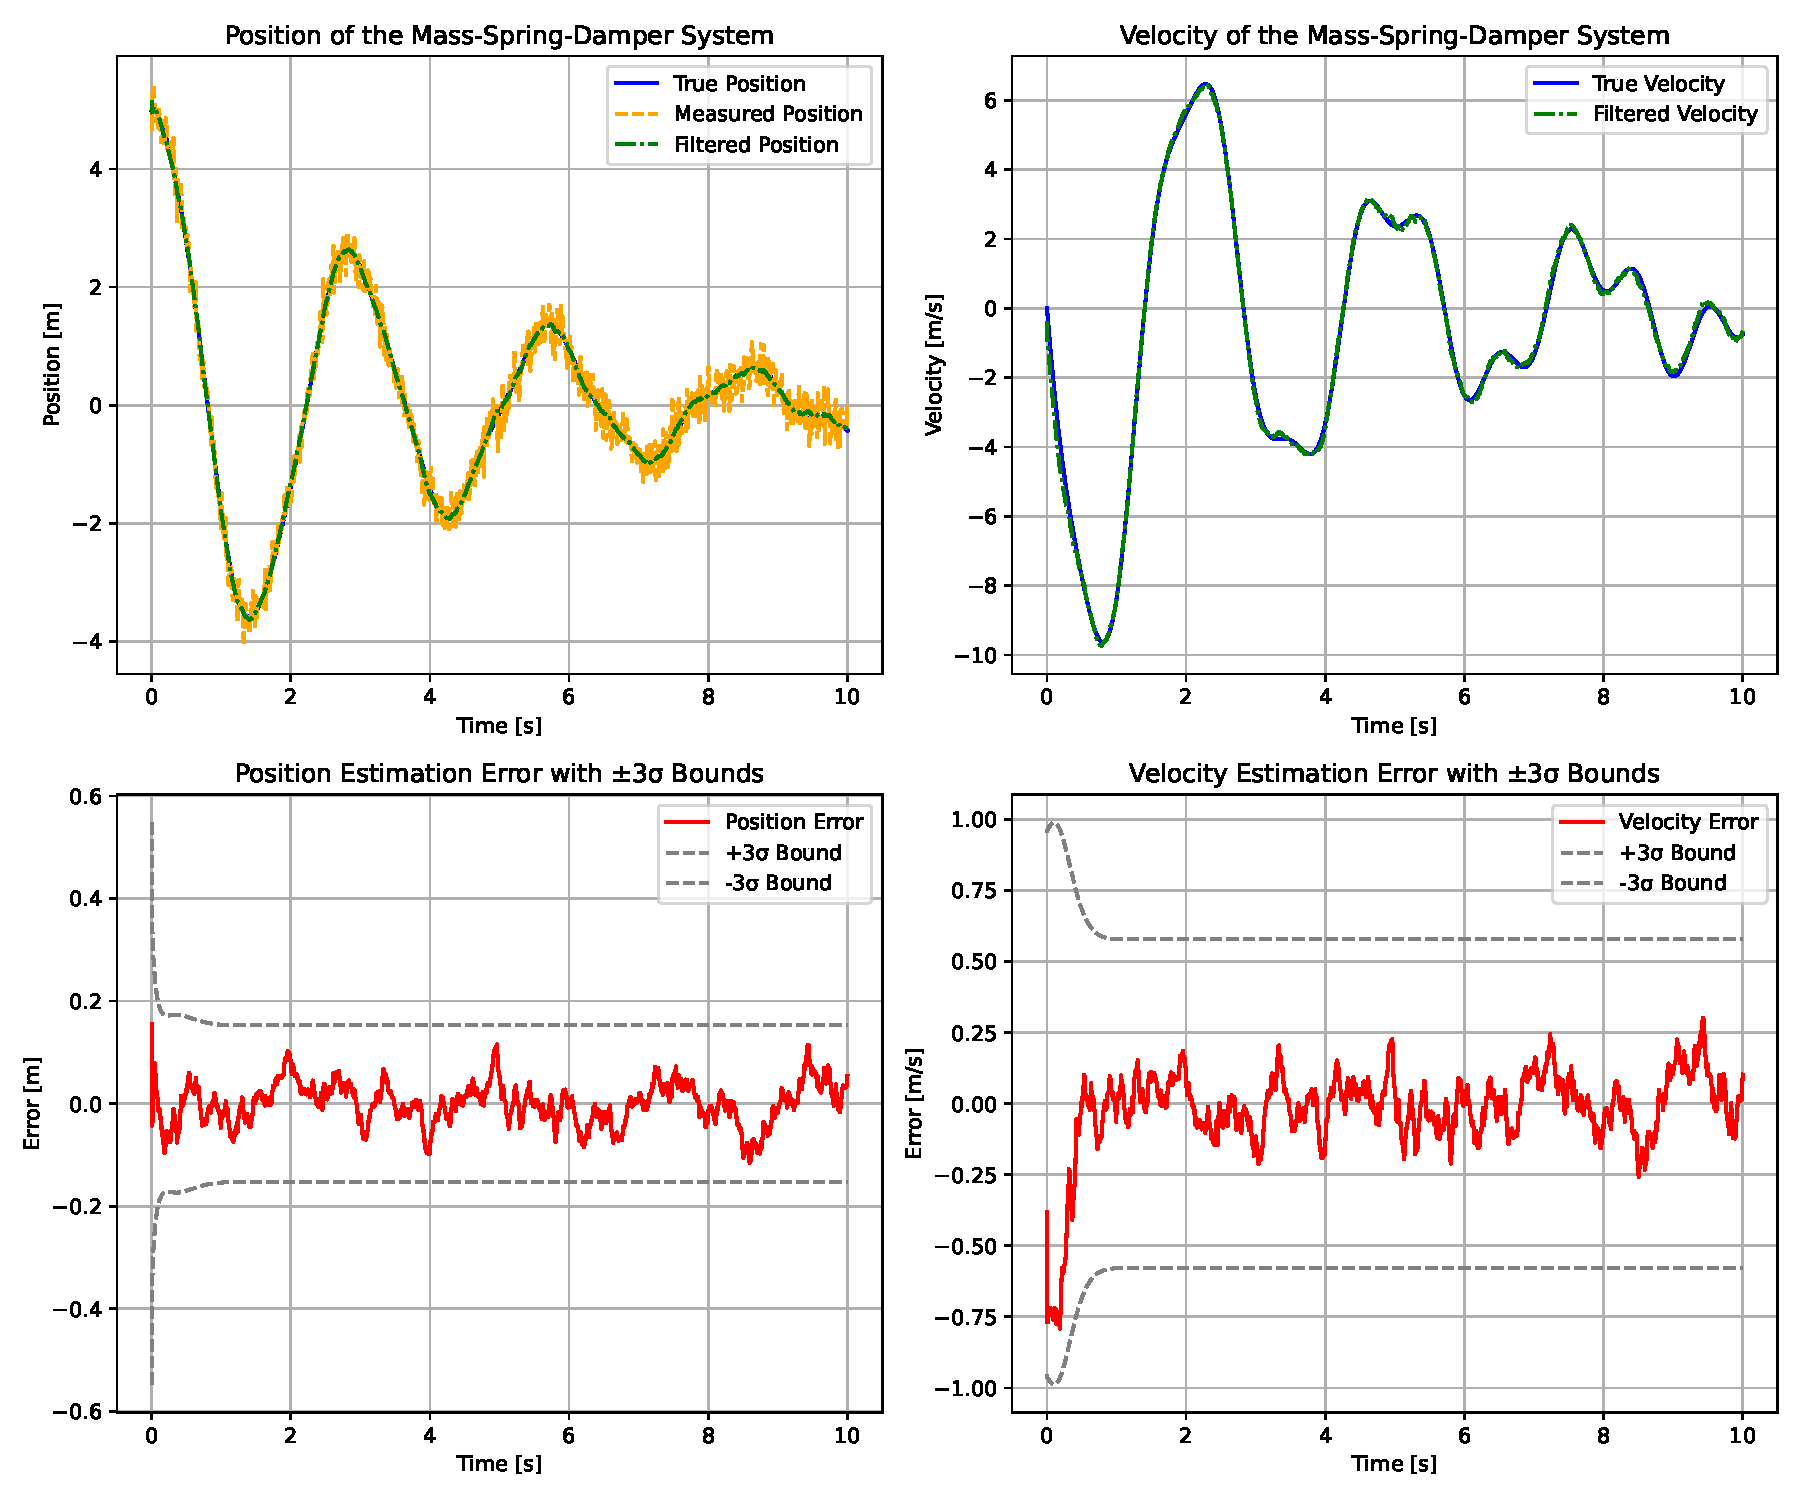
\includegraphics[width=1\textwidth]{figures/kf_same_freq.pdf}
    \caption{Kalman filter estimation with accelerometer and position measurements at the same frequency. The plots show the true, measured, and filtered values for position and velocity, as well as the errors with $\pm 3\sigma$ bounds.}
    \label{fig:kf_same_freq}
\end{figure}

The figure above demonstrates the performance of the Kalman filter when both accelerometer  
and position measurements are sampled at the same frequency. The filter effectively fuses  
the two sources to provide accurate estimates with uncertainty bounds.

In Figure \ref{fig:kf_freq_50}, the accelerometer data is sampled 50 times more frequently  
than the position measurements. Between two position updates, the filter relies solely on  
the accelerometer data to predict the state. This causes the state covariance to increase as  
uncertainty accumulates. When a position measurement becomes available, the update step  
reduces the uncertainty, resulting in a drop in the covariance. This cycle repeats, and the  
error bounds expand and contract periodically, reflecting the alternating prediction-only  
and correction phases.

\begin{figure}[H]
    \centering
    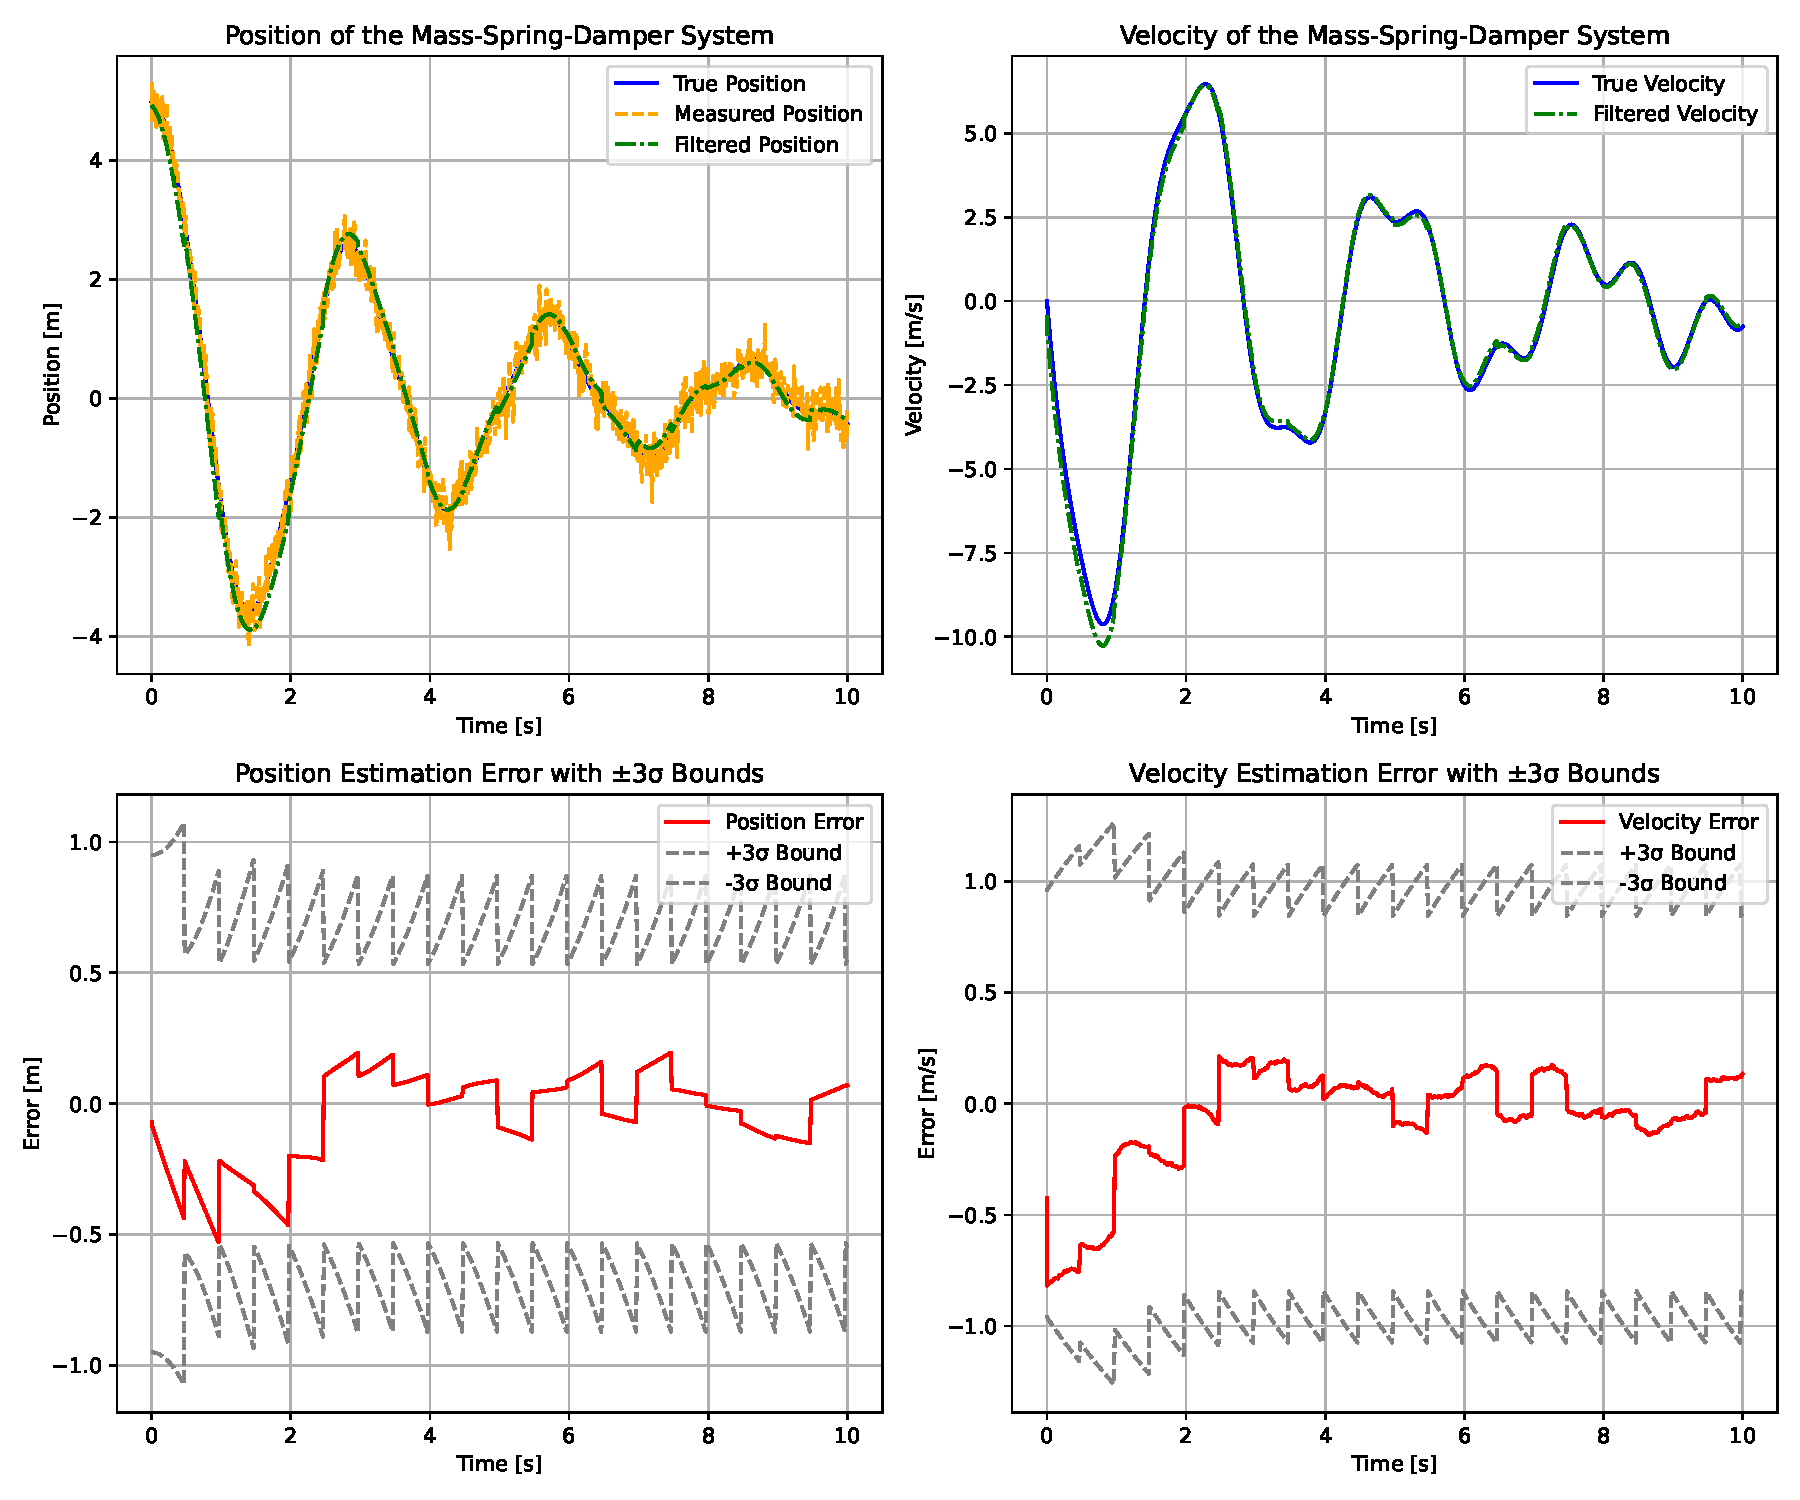
\includegraphics[width=1\textwidth]{figures/kf_freq_50.pdf}
    \caption{Kalman filter estimation where the accelerometer is sampled 50 times more frequently than the position sensor.}
    \label{fig:kf_freq_50}
\end{figure}

